%# -*- coding: utf-8 -*-
%!TEX encoding = UTF-8 Unicode
%!TEX TS-program = xelatex
% vim:ts=4:sw=4
%
% 以上设定默认使用 XeLaTex 编译,并指定 Unicode 编码,供 TeXShop 自动识别

% Author: Yunhui Fu <yhfudev@gmail.com>
% License: Creative Commons (CC BY 4.0)

\section{\cnt{Self-Taught Learning and Unsupervised Feature Learning}{自我学习与无监督特征学习}{}} \label{chp:selftaughtlearning}

\subsection{\cnt{Self-Taught Learning}{自我学习}{}}

\subsubsection{\cnt{Overview}{综述}{}}

\cnt{Assuming that we have a sufficiently powerful learning algorithm, one of the most reliable ways to get better performance is to give the algorithm more data. This has led to the that aphorism that in machine learning, ``sometimes it's not who has the best algorithm that wins; it's who has the most data." }
    {如果已经有一个足够强大的机器学习算法,为了获得更好的性能,最靠谱的方法之一是给这个算法以更多的数据。机器学习界甚至有个说法:“有时候胜出者并非有最好的算法,而是有更多的数据。” }
    {}


\cnt{One can always try to get more labeled data, but this can be expensive. In particular, researchers have already gone to extraordinary lengths to use tools such as AMT (Amazon Mechanical Turk) to get large training sets. While having large numbers of people hand-label lots of data is probably a step forward compared to having large numbers of researchers hand-engineer features, it would be nice to do better. In particular, the promise of \emph{self-taught learning} and \emph{unsupervised feature learning} is that if we can get our algorithms to learn from unlabeled data, then we can easily obtain and learn from massive amounts of it. Even though a single unlabeled example is less informative than a single labeled example, if we can get tons of the former---for example, by downloading random unlabeled images/audio clips/text documents off the internet---and if our algorithms can exploit this unlabeled data effectively, then we might be able to achieve better performance than the massive hand-engineering and massive hand-labeling approaches. }
    {人们总是可以尝试获取更多的已标注数据,但是这样做成本往往很高。例如研究人员已经花了相当的精力在使用类似 AMT(Amazon Mechanical Turk) 这样的工具上,以期获取更大的训练数据集。相比大量研究人员通过手工方式构建特征,用众包的方式让多人手工标数据是一个进步,但是我们可以做得更好。具体的说,如果算法能够从未标注数据中学习,那么我们就可以轻易地获取大量无标注数据,并从中学习。自学习和无监督特征学习就是这种的算法。尽管一个单一的未标注样本蕴含的信息比一个已标注的样本要少,但是如果能获取大量无标注数据(比如从互联网上下载随机的、无标注的图像、音频剪辑或者是文本),并且算法能够有效的利用它们,那么相比大规模的手工构建特征和标数据,算法将会取得更好的性能。 }
    {}


\cnt{In Self-taught learning and Unsupervised feature learning, we will give our algorithms a large amount of unlabeled data with which to learn a good feature representation of the input. If we are trying to solve a specific classification task, then we take this learned feature representation and whatever (perhaps small amount of) labeled data we have for that classification task, and apply supervised learning on that labeled data to solve the classification task. }
    {在自学习和无监督特征学习问题上,可以给算法以大量的未标注数据,学习出较好的特征描述。在尝试解决一个具体的分类问题时,可以基于这些学习出的特征描述和任意的(可能比较少的)已标注数据,使用有监督学习方法完成分类。 }
    {}


\cnt{These ideas probably have the most powerful effects in problems where we have a lot of unlabeled data, and a smaller amount of labeled data. However, they typically give good results even if we have only labeled data (in which case we usually perform the feature learning step using the labeled data, but ignoring the labels). }
    {在一些拥有大量未标注数据和少量的已标注数据的场景中,上述思想可能是最有效的。即使在只有已标注数据的情况下(这时我们通常忽略训练数据的类标号进行特征学习),以上想法也能得到很好的结果。 }
    {}


\subsubsection{\cnt{Learning features}{特征学习}{}}

\cnt{We have already seen how an autoencoder can be used to learn features from unlabeled data. Concretely, suppose we have an unlabeled training set $\{ x_u^{(1)}, x_u^{(2)}, \ldots, x_u^{(m_u)}\}$ with $m_u$ unlabeled examples. (The subscript ``u" stands for ``unlabeled.") We can then train a sparse autoencoder on this data (perhaps with appropriate whitening or other pre-processing): }
    {我们已经了解到如何使用一个自编码器(autoencoder)从无标注数据中学习特征。具体来说,假定有一个无标注的训练数据集 $\{ x_u^{(1)}, x_u^{(2)}, \ldots, x_u^{(m_u)}\}$(下标 $u$ 代表“不带类标”)。现在用它们训练一个稀疏自编码器(可能需要首先对这些数据做白化或其它适当的预处理)。 }
    {}

\begin{figure}[ht] \centering
  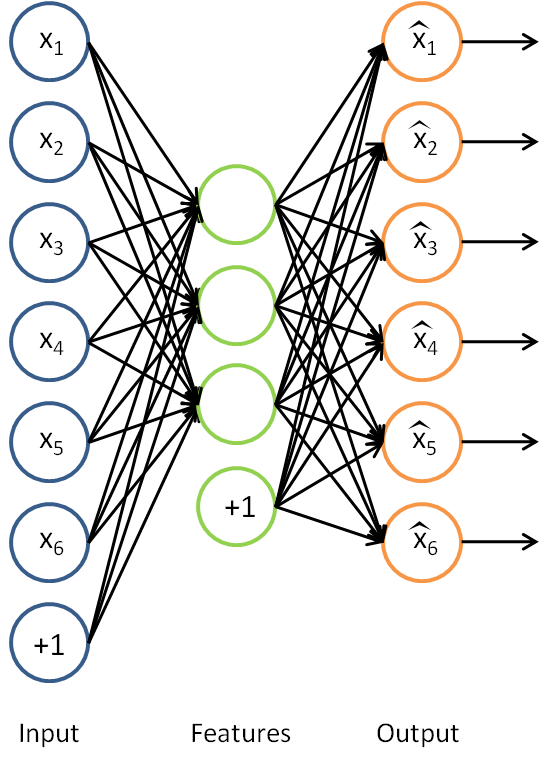
\includegraphics[width=0.4\textwidth]{figures/STL_SparseAE.png}
  %\caption{}\label{fig:zcawhiten}
\end{figure}

\cnt{Having trained the parameters $W^{(1)}, b^{(1)}, W^{(2)}, b^{(2)}$ of this model, given any new input $x$, we can now compute the corresponding vector of activations $a$ of the hidden units. As we saw previously, this often gives a better representation of the input than the original raw input $x$. We can also visualize the algorithm for computing the features/activations $a$ as the following neural network: }
    {利用训练得到的模型参数 $W^{(1)}, b^{(1)}, W^{(2)}, b^{(2)}$,给定任意的输入数据 $x$,可以计算隐藏单元的激活量(activations) $a$。如前所述,相比原始输入 $x$ 来说,$a$ 可能是一个更好的特征描述。下图的神经网络描述了特征(激活量 $a$)的计算。 }
    {}

\begin{figure}[ht] \centering
  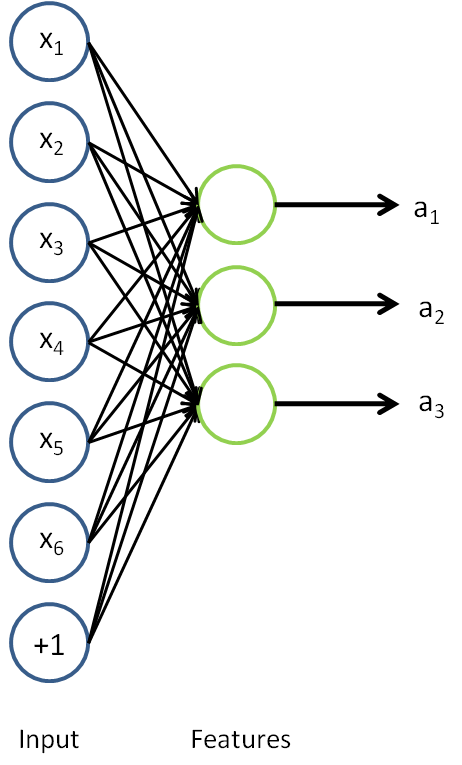
\includegraphics[width=0.4\textwidth]{figures/STL_SparseAE_Features.png}
  %\caption{}\label{fig:zcawhiten}
\end{figure}

\cnt{This is just the sparse autoencoder that we previously had, with with the final layer removed. }
    {这实际上就是之前得到的稀疏自编码器,在这里去掉了最后一层。}
    {}

\cnt{Now, suppose we have a labeled training set $\{ (x_l^{(1)}, y^{(1)}), (x_l^{(2)}, y^{(2)}), \ldots (x_l^{(m_l)}, y^{(m_l)}) \}$ of $m_l$ examples. (The subscript ``$l$" stands for ``labeled.") We can now find a better representation for the inputs. In particular, rather than representing the first training example as $x_l^{(1)}$, we can feed $x_l^{(1)}$ as the input to our autoencoder, and obtain the corresponding vector of activations $a_l^{(1)}$. To represent this example, we can either just \emph{replace} the original feature vector with $a_l^{(1)}$. Alternatively, we can \emph{concatenate} the two feature vectors together, getting a representation $(x_l^{(1)}, a_l^{(1)})$. }
    {假定有大小为 $m_l$ 的已标注训练集 $\{ (x_l^{(1)}, y^{(1)}), (x_l^{(2)}, y^{(2)}), \ldots (x_l^{(m_l)}, y^{(m_l)}) \}$(下标 $l$ 表示“带类标”),我们可以为输入数据找到更好的特征描述。例如,可以将 $x_l^{(1)}$ 输入到稀疏自编码器,得到隐藏单元激活量 $a_l^{(1)}$。接下来,可以直接使用 $a_l^{(1)}$ 来\emph{代替}原始数据 $x_l^{(1)}$ (“替代表示”,Replacement Representation)。也可以合二为一,使用新的向量 $(x_l^{(1)}, a_l^{(1)})$ 来代替原始数据 $x_l^{(1)}$ (“级联表示”,Concatenation Representation)。 }
    {}

\cnt{Thus, our training set now becomes $\{ (a_l^{(1)}, y^{(1)}), (a_l^{(2)}, y^{(2)}), \ldots (a_l^{(m_l)}, y^{(m_l)}) \}$ (if we use the replacement representation, and use $a_l^{(i)}$ to represent the $i$-th training example), or $\{ ((x_l^{(1)}, a_l^{(1)}), y^{(1)}), ((x_l^{(2)}, a_l^{(1)}), y^{(2)}), \ldots, ((x_l^{(m_l)}, a_l^{(1)}), y^{(m_l)}) \}$ (if we use the concatenated representation). In practice, the concatenated representation often works better; but for memory or computation representations, we will sometimes use the replacement representation as well. }
    {经过变换后,训练集就变成 $\{ (a_l^{(1)}, y^{(1)}), (a_l^{(2)}, y^{(2)}), \ldots (a_l^{(m_l)}, y^{(m_l)}) \}$ 或者是 $\{ ((x_l^{(1)}, a_l^{(1)}), y^{(1)}), ((x_l^{(2)}, a_l^{(1)}), y^{(2)}), \ldots, ((x_l^{(m_l)}, a_l^{(1)}), y^{(m_l)}) \}$(取决于使用 $a_l^{(1)}$ 替换 $x_l^{(1)}$ 还是将二者合并)。在实践中,将 $a_l^{(1)}$ 和 $x_l^{(1)}$ 合并通常表现的更好。但是考虑到内存和计算的成本,也可以使用替换操作。 }
    {}

\cnt{Finally, we can train a supervised learning algorithm such as an SVM, logistic regression, etc. to obtain a function that makes predictions on the $y$ values. Given a test example $x_{\rm test}$, we would then follow the same procedure: For feed it to the autoencoder to get $a_{\rm test}$. Then, feed either $a_{\rm test}$ or $(x_{\rm test}, a_{\rm test})$ to the trained classifier to get a prediction. }
    {最终,可以训练出一个有监督学习算法(例如 svm, logistic regression 等),得到一个判别函数对 $y$ 值进行预测。预测过程如下:给定一个测试样本 $x_{\rm test}$,重复之前的过程,将其送入稀疏自编码器,得到 $a_{\rm test}$。然后将 $a_{\rm test}$ (或者 $(x_{\rm test}, a_{\rm test})$ )送入分类器中,得到预测值。 }
    {}

\subsubsection{\cnt{On pre-processing the data}{数据预处理}{}}

\cnt{During the feature learning stage where we were learning from the unlabeled training set $\{ x_u^{(1)}, x_u^{(2)}, \ldots, x_u^{(m_u)}\}$, we may have computed various pre-processing parameters. For example, one may have computed a mean value of the data and subtracted off this mean to perform mean normalization, or used PCA to compute a matrix $U$ to represent the data as $U^Tx$ (or used PCA whitening or ZCA whitening). If this is the case, then it is important to save away these preprocessing parameters, and to use the same parameters during the labeled training phase and the test phase, so as to make sure we are always transforming the data the same way to feed into the autoencoder. In particular, if we have computed a matrix $U$ using the unlabeled data and PCA, we should keep the same matrix $U$ and use it to preprocess the labeled examples and the test data. We should not re-estimate a different $U$ matrix (or data mean for mean normalization, etc.) using the labeled training set, since that might result in a dramatically different pre-processing transformation, which would make the input distribution to the autoencoder very different from what it was actually trained on. }
    {在特征学习阶段,我们从未标注训练集 $\{ x_u^{(1)}, x_u^{(2)}, \ldots, x_u^{(m_u)}\}$ 中学习,这一过程中可能计算了各种数据预处理参数。例如计算数据均值并且对数据做均值标准化(mean normalization);或者对原始数据做主成分分析(PCA),然后将原始数据表示为 $U^Tx$ (又或者使用 PCA 白化或 ZCA 白化)。这样的话,有必要将这些参数保存起来,并且在后面的训练和测试阶段使用同样的参数,以保证数据进入稀疏自编码神经网络之前经过了同样的变换。例如,如果对未标注数据集进行PCA预处理,就必须将得到的矩阵 $U$ 保存起来,并且应用到有标注训练集和测试集上;而不能使用有标注训练集重新估计出一个不同的矩阵 $U$ (也不能重新计算均值并做均值标准化),否则的话可能得到一个完全不一致的数据预处理操作,导致进入自编码器的数据分布迥异于训练自编码器时的数据分布。 }
    {}

\subsubsection{\cnt{On the terminology of unsupervised feature learning }{无监督特征学习的术语}{}}

\cnt{There are two common unsupervised feature learning settings, depending on what type of unlabeled data you have. The more general and powerful setting is the \emph{self-taught learning} setting, which does not assume that your unlabeled data $x_u$ has to be drawn from the same distribution as your labeled data $x_l$. The more restrictive setting where the unlabeled data comes from exactly the same distribution as the labeled data is sometimes called the \emph{semi-supervised learning} setting. This distinctions is best explained with an example, which we now give. }
    {有两种常见的无监督特征学习方式,区别在于你有什么样的未标注数据。\emph{自学习}(self-taught learning) 是其中更为一般的、更强大的学习方式,它不要求未标注数据 $x_u$ 和已标注数据 $x_l$ 来自同样的分布。另外一种带限制性的方式也被称为\emph{半监督学习},它要求 $x_u$ 和 $x_l$ 服从同样的分布。下面通过例子解释二者的区别。 }
    {}

\cnt{Suppose your goal is a computer vision task where you'd like to distinguish between images of cars and images of motorcycles; so, each labeled example in your training set is either an image of a car or an image of a motorcycle. Where can we get lots of unlabeled data? The easiest way would be to obtain some random collection of images, perhaps downloaded off the internet. We could then train the autoencoder on this large collection of images, and obtain useful features from them. Because here the unlabeled data is drawn from a different distribution than the labeled data (i.e., perhaps some of our unlabeled images may contain cars/motorcycles, but not every image downloaded is either a car or a motorcycle), we call this self-taught learning. }
    {假定有一个计算机视觉方面的任务,目标是区分汽车和摩托车图像;也即训练样本里面要么是汽车的图像,要么是摩托车的图像。哪里可以获取大量的未标注数据呢?最简单的方式可能是从互联网上下载一些随机的图像数据集,在这些数据上训练出一个稀疏自编码器,从中得到有用的特征。这个例子里,未标注数据完全来自于一个和已标注数据不同的分布(未标注数据集中,或许其中一些图像包含汽车或者摩托车,但是不是所有的图像都如此)。这种情形被称为自学习。 }
    {}

\cnt{In contrast, if we happen to have lots of unlabeled images lying around that are all images of either a car or a motorcycle, but where the data is just missing its label (so you don't know which ones are cars, and which ones are motorcycles), then we could use this form of unlabeled data to learn the features. This setting---where each unlabeled example is drawn from the same distribution as your labeled examples---is sometimes called the semi-supervised setting. In practice, we often do not have this sort of unlabeled data (where would you get a database of images where every image is either a car or a motorcycle, but just missing its label?), and so in the context of learning features from unlabeled data, the self-taught learning setting is more broadly applicable. }
    {相反,如果有大量的未标注图像数据,要么是汽车图像,要么是摩托车图像,仅仅是缺失了类标号(没有标注每张图片到底是汽车还是摩托车)。也可以用这些未标注数据来学习特征。这种方式,即要求未标注样本和带标注样本服从相同的分布,有时候被称为半监督学习。在实践中,常常无法找到满足这种要求的未标注数据(到哪里找到一个每张图像不是汽车就是摩托车,只是丢失了类标号的图像数据库?)因此,自学习在无标注数据集的特征学习中应用更广。 }
    {}

\subsection{\cnt{Exercise: Self-Taught Learning}{练习:自学习}{}} \label{chp:execselftaughtlearn}

\subsubsection{\cnt{Overview}{综述}{}}

\cnt{In this exercise, we will use the self-taught learning paradigm with the sparse autoencoder and softmax classifier to build a classifier for handwritten digits. }
    {}
    {}


\cnt{You will be building upon your code from the earlier exercises. First, you will train your sparse autoencoder on an ``unlabeled" training dataset of handwritten digits. This produces feature that are penstroke-like. We then extract these learned features from a labeled dataset of handwritten digits. These features will then be used as inputs to the softmax classifier that you wrote in the previous exercise. }
    {}
    {}


\cnt{Concretely, for each example in the the labeled training dataset $x_l$, we forward propagate the example to obtain the activation of the hidden units $a^{(2)}$. We now represent this example using $a^{(2)}$ (the ``replacement" representation), and use this to as the new feature representation with which to train the softmax classifier. }
    {}
    {}


\cnt{Finally, we also extract the same features from the test data to obtain predictions.}
    {}
    {}

\cnt{In this exercise, our goal is to distinguish between the digits from 0 to 4. We will use the digits 5 to 9 as our ``unlabeled" dataset which which to learn the features; we will then use a labeled dataset with the digits 0 to 4 with which to train the softmax classifier.}
    {}
    {}

\cnt{In the starter code, we have provided a file \texttt{stlExercise.m} that will help walk you through the steps in this exercise. }
    {}
    {}

\subsubsection{\cnt{Dependencies}{}{}}

\cnt{The following additional files are required for this exercise: }
    {}
    {}
\begin{itemize}
  \item MNIST Dataset \url{http://yann.lecun.com/exdb/mnist/}
  \item Support functions for loading MNIST in Matlab (\ref{chp:usemnistdata})
  \item Starter Code \href{http://ufldl.stanford.edu/wiki/resources/stl_exercise.zip}{stl\_exercise.zip}) 
\end{itemize}

\cnt{You will also need your code from the following exercises: }
    {}
    {}
\begin{itemize}
  \item Exercise:Sparse Autoencoder (\ref{chp:execsparseautoenc})
  \item Exercise:Vectorization (\ref{chp:vecexec})
  \item Exercise:Softmax Regression (\ref{chp:execsoftmaxreg})
\end{itemize}

\emph{
\cnt{If you have not completed the exercises listed above, we strongly suggest you complete them first.}
    {}
    {}
}

\subsubsection{\cnt{Step 1: Generate the input and test data sets}{}{}}

\cnt{Download and decompress \href{http://ufldl.stanford.edu/wiki/resources/stl_exercise.zip}{stl\_exercise.zip}, which contains starter code for this exercise. Additionally, you will need to download the datasets from the MNIST Handwritten Digit Database for this project. }
    {}
    {}

\subsubsection{\cnt{Step 2: Train the sparse autoencoder}{}{}}

\cnt{Next, use the unlabeled data (the digits from 5 to 9) to train a sparse autoencoder, using the same \texttt{sparseAutoencoderCost.m} function as you had written in the previous exercise. (From the earlier exercise, you should have a working and vectorized implementation of the sparse autoencoder.) For us, the training step took less than 25 minutes on a fast desktop. When training is complete, you should get a visualization of pen strokes like the image shown below: }
    {}
    {}

\begin{figure}[ht] \centering
  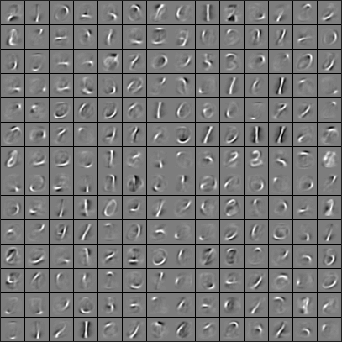
\includegraphics[width=0.5\textwidth]{figures/SelfTaughtFeatures.png}
  %\caption{}\label{fig:step1}
\end{figure}

\cnt{Informally, the features learned by the sparse autoencoder should correspond to penstrokes. }
    {}
    {}

\subsubsection{\cnt{Step 3: Extracting features}{}{}}

\cnt{After the sparse autoencoder is trained, you will use it to extract features from the handwritten digit images.}
    {}
    {}

\cnt{Complete \texttt{feedForwardAutoencoder.m} to produce a matrix whose columns correspond to activations of the hidden layer for each example, i.e., the vector $a^{(2)}$ corresponding to activation of layer 2. (Recall that we treat the inputs as layer 1).}
    {}
    {}

\cnt{After completing this step, calling \texttt{feedForwardAutoencoder.m} should convert the raw image data to hidden unit activations $a^{(2)}$.}
    {}
    {}

\subsubsection{\cnt{Step 4: Training and testing the logistic regression model}{}{}}

\cnt{Use your code from the softmax exercise (\texttt{softmaxTrain.m}) to train a softmax classifier using the training set features (\texttt{trainFeatures}) and labels (\texttt{trainLabels}). }
    {}
    {}

\subsubsection{\cnt{Step 5: Classifying on the test set}{}{}}

\cnt{Finally, complete the code to make predictions on the test set (\texttt{testFeatures}) and see how your learned features perform! If you've done all the steps correctly, you should get an accuracy of about 98\% percent. }
    {}
    {}

\cnt{As a comparison, when \emph{raw pixels} are used (instead of the learned features), we obtained a test accuracy of only around 96\% (for the same train and test sets). }
    {}
    {}
